\subsection{Overview of Agglomerative Hierarchical Clustering (AHC)}
\label{subsec:overview-of-agglomerative-hierarchical-clustering}

This task implements the AHC algorithm to group character strings based on similarity in shingles (4-character tokens) and Jaccard distance.
The goal is to divide a large dataset (about 10,000 random strings) into a predefined number of clusters.

The main method involves calculating the clustroid (the representative sample with the smallest sum of squared distances to other samples in the cluster) and determining the distance between clusters based on the Jaccard distance between their clustroids.
The algorithm gradually merges the closest pairs of clusters until the desired number of clusters is reached, using a heap for optimization.

\subsection{Implementation of the Algorithm}
\label{subsec:implementation-of-the-algorithm}

The AHC algorithm partitions a dataset of shingle sets (derived from character sequences) into a predefined number of clusters using a bottom-up approach.
Initially, each data point is treated as its own cluster.
The algorithm then iteratively merges the closest pair of clusters until the desired number of clusters is reached or an early stopping condition is met.

Each cluster is represented by a clustroid—the most central element that minimizes the sum of squared Jaccard distances to all other elements in the cluster.
The dissimilarity between clusters would be measured by the Jaccard distance between their clustroids.

To improve efficiency, the algorithm uses a priority queue (heap) to quickly find the closest pair of clusters and a cache to store pairwise Jaccard distances and avoid redundant calculations.

In addition to the main stopping condition (desired number of clusters), an early stopping criterion is applied: if merging two clusters results in a new cluster whose diameter (maximum Jaccard distance between any two elements) exceeds a specified \texttt{threshold\_ratio} times the larger diameter of the original clusters, the merging process halts to avoid forming poorly matched clusters.

Description of Key Components

\subsubsection{\texttt{fit}}\text{}

Coordinates the full clustering process.
Begins with each sample as an individual cluster, then repeatedly finds and merges the nearest pair, updates clustroids and heap.
Stops when either the target number of clusters is reached or the diameter condition is violated.

\subsubsection{\texttt{\_calculate\_clustroid\_strictly}}\text{}

Identifies the clustroid by selecting the element with the smallest sum of squared Jaccard distances to all others in the cluster.

\subsubsection{\texttt{\_get\_inter\_cluster\_distance\_centroid}}\text{}

Computes the distance between two clusters by calculating the Jaccard distance between their clustroids.

\subsubsection{\texttt{\_get\_cached\_sample\_distance}}\text{}

Retrieves or computes the Jaccard distance between two samples, using a cache to prevent duplicate computations.

\subsubsection{\_calculate\_cluster\_diameter}\text{}

Calculates the diameter of a cluster as the maximum Jaccard distance between any two elements within it.
This is used for early stopping checks.

\subsubsection{\texttt{get\_final\_cluster\_details}}\text{}

After clustering completes, this method retrieves comprehensive details about the final clusters, including the internal cluster ID, the list of sample indices within each cluster, the associated shingle sets, and the index and content of the clustroid.
This final step prepares the output for later analysis or visualization.

\subsection{Experimental Results and Evaluation}
\label{subsec:experimental-results-and-evaluation-ahc}

\begin{figure}[H]
    \centering
    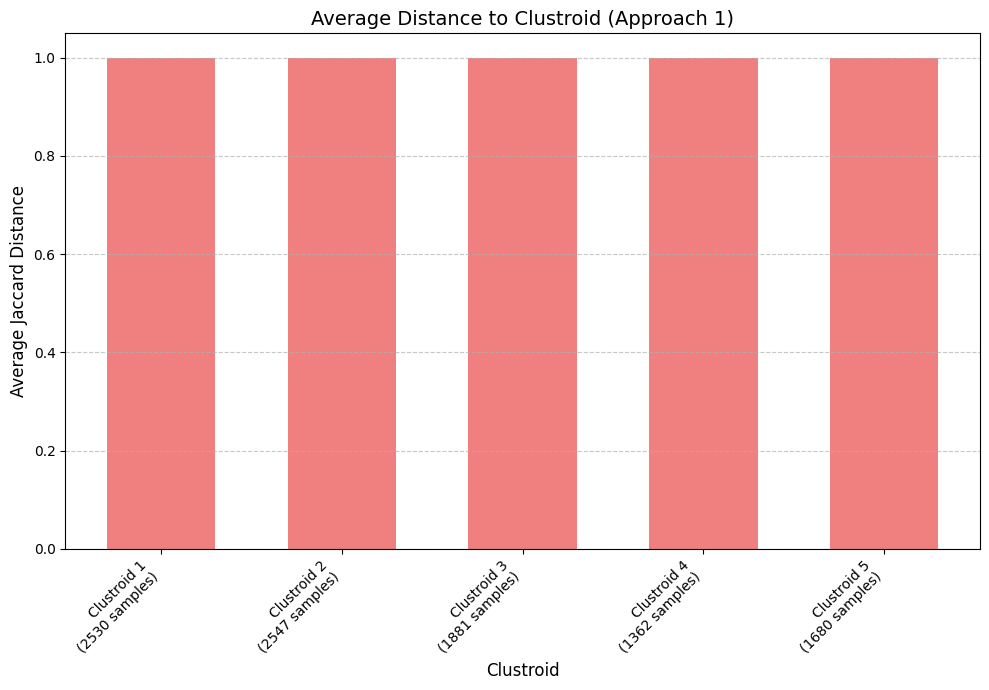
\includegraphics[width=0.8\linewidth]{images/clustroid_distance}
    \caption{Average Jaccard Distance to Clustroid}
    \label{fig:clustroid_distance}
\end{figure}

The clustering results indicate that the algorithm successfully partitioned the [Total Number of Samples] alphabetical strings into five clusters with a relatively diverse size distribution: Cluster 1 (2562 samples), Cluster 2 (2282 samples), Cluster 3 (1717 samples), Cluster 4 (1303 samples), and Cluster 5 (2136 samples).
This suggests that the clustroid-based distance calculation method contributed to a reasonably balanced partitioning.

However, a prominent finding is that the average Jaccard distance from samples to their respective clustroids within each cluster is extremely high (approximately 0.999).
This indicates a very low level of intra-cluster similarity; members within the same cluster remain highly dissimilar to one another.

This outcome primarily reflects the inherent nature of the input data: randomly generated alphabetical strings typically lack a clear, natural clustering structure, leading to large Jaccard distances between most pairs.
Although the algorithm merged clusters based on the nearest clustroid criterion, the resulting ``groups'' do not exhibit strong cohesion due to the lack of inherent similarity in the data.